\documentclass{standalone}
\usepackage{tikz}
\usetikzlibrary{patterns, positioning}
\usepackage[sfdefault]{ClearSans} %% option 'sfdefault' activates Clear Sans as the default text font
\usepackage[T1]{fontenc}

\begin{document}
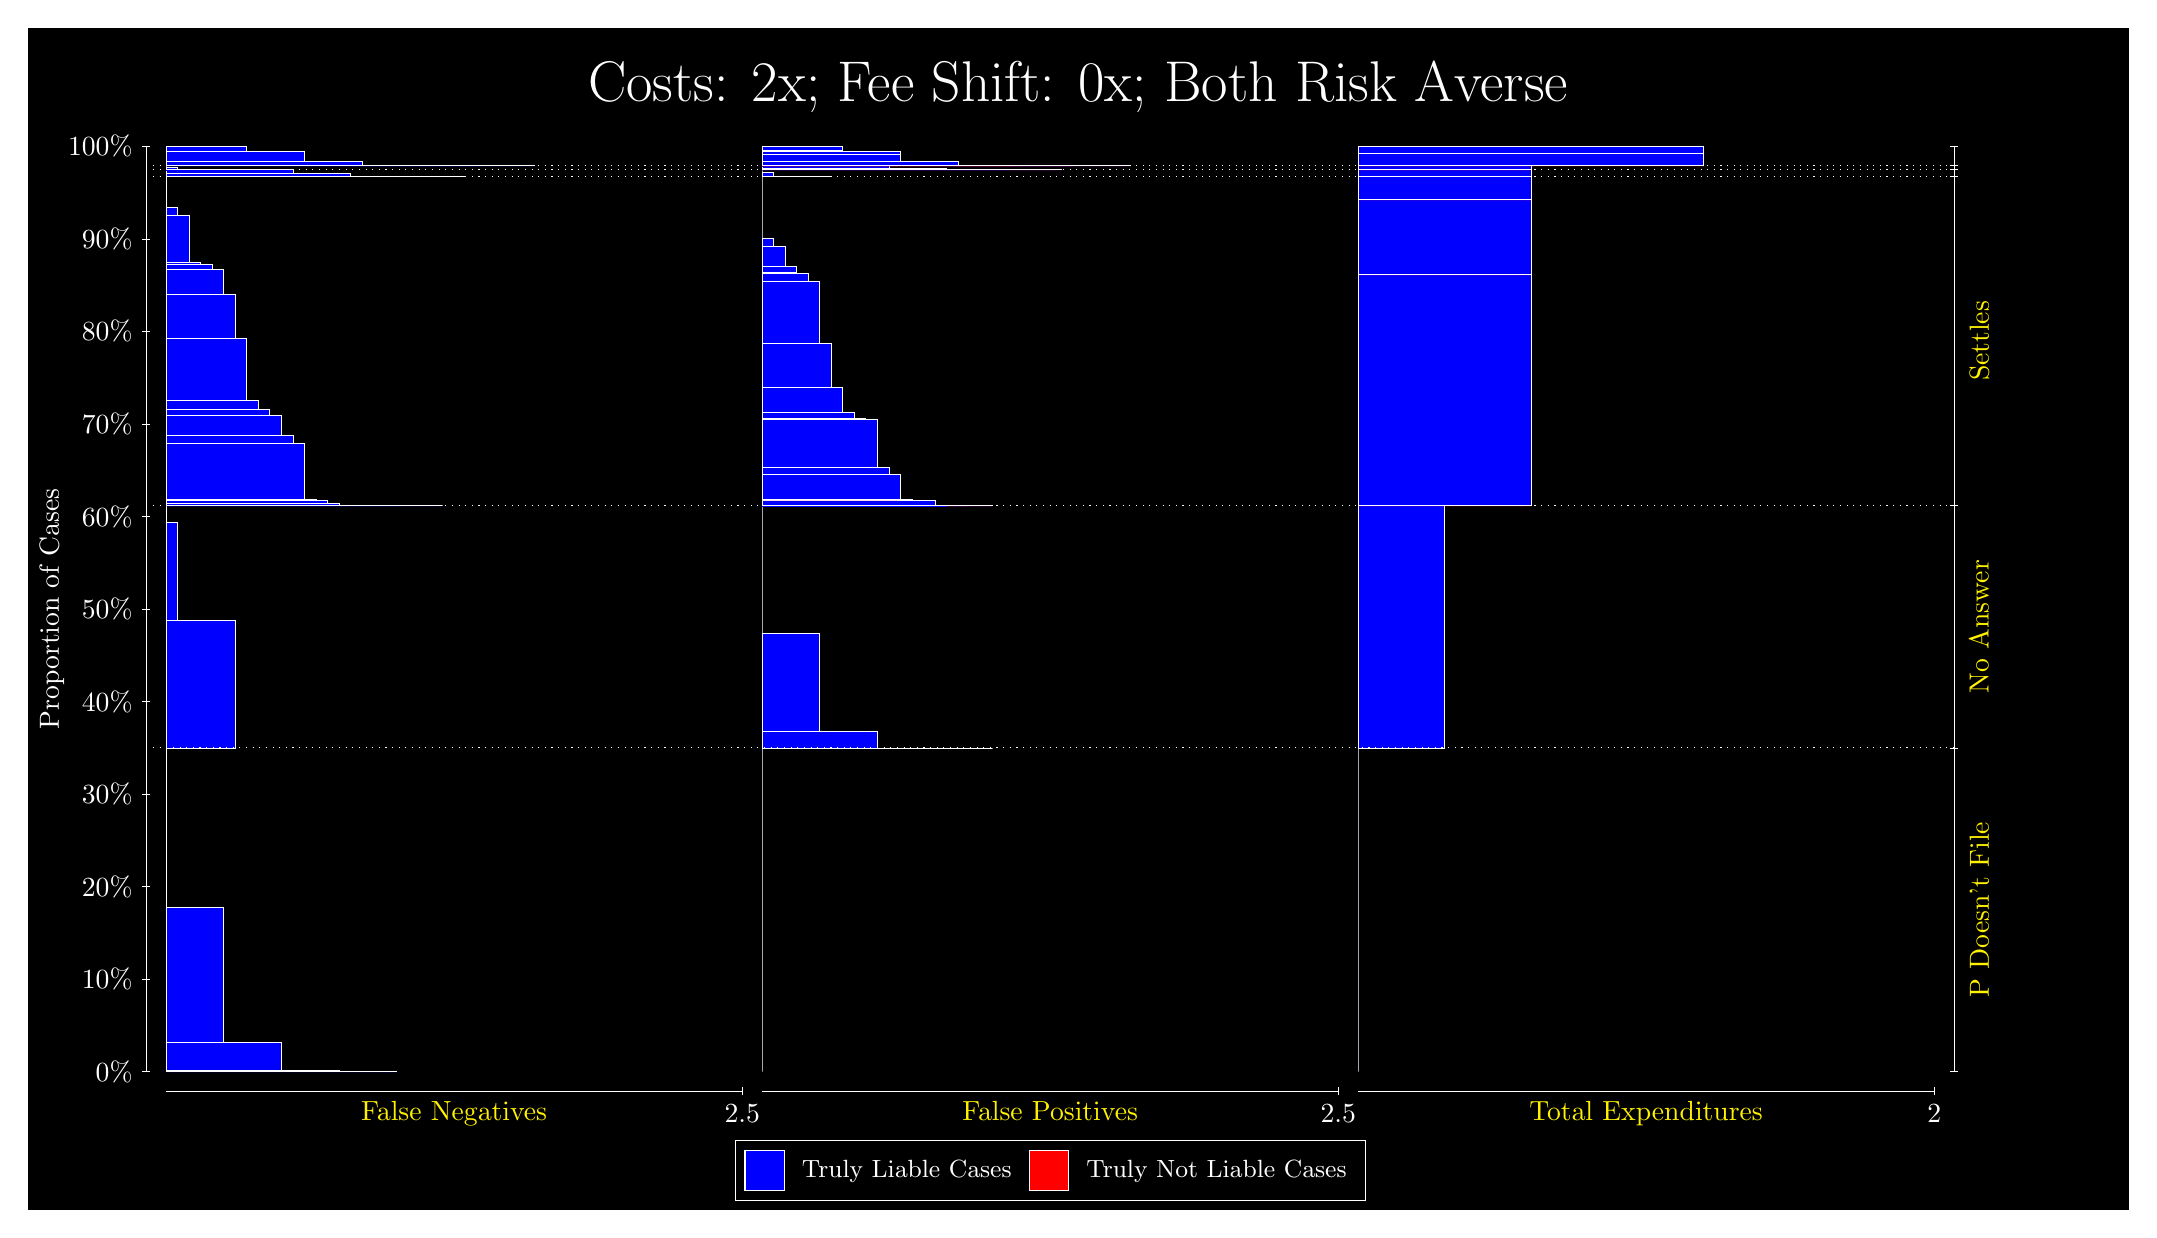
\begin{tikzpicture}
\draw[fill=black] (0,0) rectangle (26.667,15);
\draw[text=white] (0,13.5) rectangle (26.667,15) node[midway] {\huge Costs: 2x; Fee Shift: 0x; Both Risk Averse};
\draw[white, very thin] (1.5,1.75) -- (1.5,13.5);
\node[rotate=90, text=white, anchor=center] at (0.3, 7.625) {Proportion of Cases};
\draw[white, very thin] (1.45,1.75) -- (1.55,1.75);
\node[text=white, anchor=east] at (1.45, 1.75) {0\%};
\draw[white, very thin] (1.45,2.925) -- (1.55,2.925);
\node[text=white, anchor=east] at (1.45, 2.925) {10\%};
\draw[white, very thin] (1.45,4.1) -- (1.55,4.1);
\node[text=white, anchor=east] at (1.45, 4.1) {20\%};
\draw[white, very thin] (1.45,5.275) -- (1.55,5.275);
\node[text=white, anchor=east] at (1.45, 5.275) {30\%};
\draw[white, very thin] (1.45,6.45) -- (1.55,6.45);
\node[text=white, anchor=east] at (1.45, 6.45) {40\%};
\draw[white, very thin] (1.45,7.625) -- (1.55,7.625);
\node[text=white, anchor=east] at (1.45, 7.625) {50\%};
\draw[white, very thin] (1.45,8.8) -- (1.55,8.8);
\node[text=white, anchor=east] at (1.45, 8.8) {60\%};
\draw[white, very thin] (1.45,9.975) -- (1.55,9.975);
\node[text=white, anchor=east] at (1.45, 9.975) {70\%};
\draw[white, very thin] (1.45,11.15) -- (1.55,11.15);
\node[text=white, anchor=east] at (1.45, 11.15) {80\%};
\draw[white, very thin] (1.45,12.325) -- (1.55,12.325);
\node[text=white, anchor=east] at (1.45, 12.325) {90\%};
\draw[white, very thin] (1.45,13.5) -- (1.55,13.5);
\node[text=white, anchor=east] at (1.45, 13.5) {100\%};

\draw[white, very thin] (24.457,1.75) -- (24.457,13.5);
\draw[white, very thin] (24.407,1.75) -- (24.507,1.75);
\node[anchor=west] at (24.407, 1.75) {};
\draw[white, very thin] (24.407,5.8604) -- (24.507,5.8604);
\node[anchor=west] at (24.407, 5.8604) {};
\draw[white, very thin] (24.407,8.9376) -- (24.507,8.9376);
\node[anchor=west] at (24.407, 8.9376) {};
\draw[white, very thin] (24.407,13.121) -- (24.507,13.121);
\node[anchor=west] at (24.407, 13.121) {};
\draw[white, very thin] (24.407,13.204) -- (24.507,13.204);
\node[anchor=west] at (24.407, 13.204) {};
\draw[white, very thin] (24.407,13.255) -- (24.507,13.255);
\node[anchor=west] at (24.407, 13.255) {};
\draw[white, very thin] (24.407,13.5) -- (24.507,13.5);
\node[anchor=west] at (24.407, 13.5) {};

\draw[white, very thin, fill=blue] (1.75,1.75) rectangle (4.6775,1.7501);
\draw[white, very thin, fill=blue] (1.75,1.7501) rectangle (3.9457,1.761);
\draw[white, very thin, fill=blue] (1.75,1.761) rectangle (3.2138,2.1187);
\draw[white, very thin, fill=blue] (1.75,2.1187) rectangle (2.4819,3.8341);
\draw[white, very thin, fill=red] (1.75,3.8341) rectangle (1.75,3.8341);
\draw[white, very thin, fill=blue] (1.75,3.8341) rectangle (1.75,5.8604);
\draw[white, very thin, fill=blue] (1.75,5.8604) rectangle (2.6283,7.4798);
\draw[white, very thin, fill=blue] (1.75,7.4798) rectangle (1.8964,8.7316);
\draw[white, very thin, fill=red] (1.75,8.7316) rectangle (1.75,8.7316);
\draw[white, very thin, fill=blue] (1.75,8.7316) rectangle (1.75,8.9376);
\draw[white, very thin, fill=blue] (1.75,8.9376) rectangle (5.2631,8.9376);
\draw[white, very thin, fill=blue] (1.75,8.9376) rectangle (4.6775,8.9377);
\draw[white, very thin, fill=blue] (1.75,8.9377) rectangle (4.5312,8.9386);
\draw[white, very thin, fill=blue] (1.75,8.9386) rectangle (4.3848,8.9386);
\draw[white, very thin, fill=blue] (1.75,8.9386) rectangle (4.092,8.939);
\draw[white, very thin, fill=blue] (1.75,8.939) rectangle (3.9457,8.9699);
\draw[white, very thin, fill=blue] (1.75,8.9699) rectangle (3.7993,9.0072);
\draw[white, very thin, fill=blue] (1.75,9.0072) rectangle (3.6529,9.0126);
\draw[white, very thin, fill=blue] (1.75,9.0126) rectangle (3.5065,9.7272);
\draw[white, very thin, fill=blue] (1.75,9.7272) rectangle (3.3602,9.8312);
\draw[white, very thin, fill=blue] (1.75,9.8312) rectangle (3.2138,10.084);
\draw[white, very thin, fill=blue] (1.75,10.084) rectangle (3.0674,10.156);
\draw[white, very thin, fill=blue] (1.75,10.156) rectangle (3.0674,10.164);
\draw[white, very thin, fill=blue] (1.75,10.164) rectangle (2.921,10.275);
\draw[white, very thin, fill=blue] (1.75,10.275) rectangle (2.7746,11.059);
\draw[white, very thin, fill=blue] (1.75,11.059) rectangle (2.6283,11.619);
\draw[white, very thin, fill=blue] (1.75,11.619) rectangle (2.4819,11.933);
\draw[white, very thin, fill=blue] (1.75,11.933) rectangle (2.3355,12.008);
\draw[white, very thin, fill=blue] (1.75,12.008) rectangle (2.3355,12.008);
\draw[white, very thin, fill=blue] (1.75,12.008) rectangle (2.1891,12.028);
\draw[white, very thin, fill=blue] (1.75,12.028) rectangle (2.0428,12.628);
\draw[white, very thin, fill=blue] (1.75,12.628) rectangle (1.8964,12.725);
\draw[white, very thin, fill=red] (1.75,12.725) rectangle (1.75,12.725);
\draw[white, very thin, fill=blue] (1.75,12.725) rectangle (1.75,13.121);
\draw[white, very thin, fill=blue] (1.75,13.121) rectangle (5.5558,13.121);
\draw[white, very thin, fill=blue] (1.75,13.121) rectangle (4.8239,13.121);
\draw[white, very thin, fill=blue] (1.75,13.121) rectangle (4.092,13.152);
\draw[white, very thin, fill=blue] (1.75,13.152) rectangle (3.3602,13.203);
\draw[white, very thin, fill=blue] (1.75,13.203) rectangle (2.6283,13.204);
\draw[white, very thin, fill=red] (1.75,13.204) rectangle (1.75,13.204);
\draw[white, very thin, fill=blue] (1.75,13.204) rectangle (2.6283,13.204);
\draw[white, very thin, fill=blue] (1.75,13.204) rectangle (1.8964,13.236);
\draw[white, very thin, fill=red] (1.75,13.236) rectangle (1.75,13.236);
\draw[white, very thin, fill=blue] (1.75,13.236) rectangle (1.75,13.255);
\draw[white, very thin, fill=blue] (1.75,13.255) rectangle (6.4341,13.255);
\draw[white, very thin, fill=blue] (1.75,13.255) rectangle (5.7022,13.255);
\draw[white, very thin, fill=blue] (1.75,13.255) rectangle (4.9703,13.259);
\draw[white, very thin, fill=blue] (1.75,13.259) rectangle (4.2384,13.316);
\draw[white, very thin, fill=blue] (1.75,13.316) rectangle (3.5065,13.439);
\draw[white, very thin, fill=blue] (1.75,13.439) rectangle (2.7746,13.496);
\draw[white, very thin, fill=blue] (1.75,13.496) rectangle (2.0428,13.5);
\draw[white, very thin, fill=red] (1.75,13.5) rectangle (1.75,13.5);
\draw[white, very thin, fill=blue] (1.75,13.5) rectangle (1.75,13.5);
\draw[white, very thin, fill=red] (9.3189,1.75) rectangle (9.3189,1.75);
\draw[white, very thin, fill=blue] (9.3189,1.75) rectangle (9.3189,5.8604);
\draw[white, very thin, fill=red] (9.3189,5.8604) rectangle (12.246,5.8604);
\draw[white, very thin, fill=blue] (9.3189,5.8604) rectangle (12.246,5.8604);
\draw[white, very thin, fill=blue] (9.3189,5.8604) rectangle (11.515,5.8614);
\draw[white, very thin, fill=blue] (9.3189,5.8614) rectangle (10.783,6.0664);
\draw[white, very thin, fill=blue] (9.3189,6.0664) rectangle (10.051,7.3182);
\draw[white, very thin, fill=blue] (9.3189,7.3182) rectangle (9.3189,8.9376);
\draw[white, very thin, fill=red] (9.3189,8.9376) rectangle (12.246,8.9376);
\draw[white, very thin, fill=blue] (9.3189,8.9376) rectangle (12.246,8.9377);
\draw[white, very thin, fill=red] (9.3189,8.9377) rectangle (11.954,8.9377);
\draw[white, very thin, fill=blue] (9.3189,8.9377) rectangle (11.954,8.9377);
\draw[white, very thin, fill=red] (9.3189,8.9377) rectangle (11.661,8.9377);
\draw[white, very thin, fill=blue] (9.3189,8.9377) rectangle (11.661,8.9381);
\draw[white, very thin, fill=blue] (9.3189,8.9381) rectangle (11.515,9.0104);
\draw[white, very thin, fill=red] (9.3189,9.0104) rectangle (11.368,9.0104);
\draw[white, very thin, fill=blue] (9.3189,9.0104) rectangle (11.368,9.0106);
\draw[white, very thin, fill=blue] (9.3189,9.0106) rectangle (11.222,9.0133);
\draw[white, very thin, fill=red] (9.3189,9.0133) rectangle (11.075,9.0133);
\draw[white, very thin, fill=blue] (9.3189,9.0133) rectangle (11.075,9.3335);
\draw[white, very thin, fill=blue] (9.3189,9.3335) rectangle (10.929,9.4299);
\draw[white, very thin, fill=blue] (9.3189,9.4299) rectangle (10.783,10.031);
\draw[white, very thin, fill=blue] (9.3189,10.031) rectangle (10.636,10.05);
\draw[white, very thin, fill=red] (9.3189,10.05) rectangle (10.49,10.05);
\draw[white, very thin, fill=blue] (9.3189,10.05) rectangle (10.49,10.05);
\draw[white, very thin, fill=blue] (9.3189,10.05) rectangle (10.49,10.125);
\draw[white, very thin, fill=blue] (9.3189,10.125) rectangle (10.344,10.439);
\draw[white, very thin, fill=blue] (9.3189,10.439) rectangle (10.197,10.999);
\draw[white, very thin, fill=blue] (9.3189,10.999) rectangle (10.051,11.783);
\draw[white, very thin, fill=blue] (9.3189,11.783) rectangle (9.9044,11.894);
\draw[white, very thin, fill=blue] (9.3189,11.894) rectangle (9.758,11.903);
\draw[white, very thin, fill=blue] (9.3189,11.903) rectangle (9.758,11.974);
\draw[white, very thin, fill=blue] (9.3189,11.974) rectangle (9.6116,12.227);
\draw[white, very thin, fill=blue] (9.3189,12.227) rectangle (9.4652,12.331);
\draw[white, very thin, fill=blue] (9.3189,12.331) rectangle (9.3189,13.121);
\draw[white, very thin, fill=red] (9.3189,13.121) rectangle (10.197,13.121);
\draw[white, very thin, fill=blue] (9.3189,13.121) rectangle (10.197,13.122);
\draw[white, very thin, fill=blue] (9.3189,13.122) rectangle (9.4652,13.173);
\draw[white, very thin, fill=blue] (9.3189,13.173) rectangle (9.3189,13.204);
\draw[white, very thin, fill=red] (9.3189,13.204) rectangle (13.125,13.204);
\draw[white, very thin, fill=blue] (9.3189,13.204) rectangle (13.125,13.204);
\draw[white, very thin, fill=blue] (9.3189,13.204) rectangle (12.393,13.204);
\draw[white, very thin, fill=blue] (9.3189,13.204) rectangle (11.661,13.223);
\draw[white, very thin, fill=blue] (9.3189,13.223) rectangle (10.929,13.254);
\draw[white, very thin, fill=blue] (9.3189,13.254) rectangle (10.197,13.255);
\draw[white, very thin, fill=red] (9.3189,13.255) rectangle (14.003,13.255);
\draw[white, very thin, fill=blue] (9.3189,13.255) rectangle (14.003,13.255);
\draw[white, very thin, fill=red] (9.3189,13.255) rectangle (13.271,13.255);
\draw[white, very thin, fill=blue] (9.3189,13.255) rectangle (13.271,13.255);
\draw[white, very thin, fill=red] (9.3189,13.255) rectangle (12.539,13.255);
\draw[white, very thin, fill=blue] (9.3189,13.255) rectangle (12.539,13.259);
\draw[white, very thin, fill=blue] (9.3189,13.259) rectangle (11.807,13.315);
\draw[white, very thin, fill=red] (9.3189,13.315) rectangle (11.807,13.315);
\draw[white, very thin, fill=blue] (9.3189,13.315) rectangle (11.807,13.316);
\draw[white, very thin, fill=blue] (9.3189,13.316) rectangle (11.075,13.403);
\draw[white, very thin, fill=red] (9.3189,13.403) rectangle (11.075,13.403);
\draw[white, very thin, fill=blue] (9.3189,13.403) rectangle (11.075,13.439);
\draw[white, very thin, fill=blue] (9.3189,13.439) rectangle (10.344,13.454);
\draw[white, very thin, fill=blue] (9.3189,13.454) rectangle (10.344,13.496);
\draw[white, very thin, fill=blue] (9.3189,13.496) rectangle (9.6116,13.496);
\draw[white, very thin, fill=blue] (9.3189,13.496) rectangle (9.6116,13.5);
\draw[white, very thin, fill=blue] (9.3189,13.5) rectangle (9.3189,13.5);
\draw[white, very thin, fill=red] (16.888,1.75) rectangle (16.888,1.75);
\draw[white, very thin, fill=blue] (16.888,1.75) rectangle (16.888,5.8604);
\draw[white, very thin, fill=red] (16.888,5.8604) rectangle (17.986,5.8604);
\draw[white, very thin, fill=blue] (16.888,5.8604) rectangle (17.986,8.9376);
\draw[white, very thin, fill=red] (16.888,8.9376) rectangle (19.083,8.9376);
\draw[white, very thin, fill=blue] (16.888,8.9376) rectangle (19.083,11.871);
\draw[white, very thin, fill=red] (16.888,11.871) rectangle (19.083,11.871);
\draw[white, very thin, fill=blue] (16.888,11.871) rectangle (19.083,12.822);
\draw[white, very thin, fill=red] (16.888,12.822) rectangle (19.083,12.822);
\draw[white, very thin, fill=blue] (16.888,12.822) rectangle (19.083,13.121);
\draw[white, very thin, fill=red] (16.888,13.121) rectangle (19.083,13.121);
\draw[white, very thin, fill=blue] (16.888,13.121) rectangle (19.083,13.204);
\draw[white, very thin, fill=red] (16.888,13.204) rectangle (19.083,13.204);
\draw[white, very thin, fill=blue] (16.888,13.204) rectangle (19.083,13.255);
\draw[white, very thin, fill=red] (16.888,13.255) rectangle (21.279,13.255);
\draw[white, very thin, fill=blue] (16.888,13.255) rectangle (21.279,13.417);
\draw[white, very thin, fill=red] (16.888,13.417) rectangle (21.279,13.417);
\draw[white, very thin, fill=blue] (16.888,13.417) rectangle (21.279,13.5);
\draw[white, dotted] (1.5,5.8604) -- (24.457,5.8604);
\draw[white, dotted] (1.5,8.9376) -- (24.457,8.9376);
\draw[white, dotted] (1.5,13.121) -- (24.457,13.121);
\draw[white, dotted] (1.5,13.204) -- (24.457,13.204);
\draw[white, dotted] (1.5,13.255) -- (24.457,13.255);
\draw[white, very thin] (1.75,1.5) -- (9.0689,1.5);
\node[text=yellow, anchor=north] at (5.4094, 1.5) {False Negatives};
\draw[white, very thin] (9.0689,1.45) -- (9.0689,1.55);
\node[text=white, anchor=north] at (9.0689, 1.45) {2.5};

\draw[white, very thin] (9.3189,1.5) -- (16.638,1.5);
\node[text=yellow, anchor=north] at (12.978, 1.5) {False Positives};
\draw[white, very thin] (16.638,1.45) -- (16.638,1.55);
\node[text=white, anchor=north] at (16.638, 1.45) {2.5};

\draw[white, very thin] (16.888,1.5) -- (24.207,1.5);
\node[text=yellow, anchor=north] at (20.547, 1.5) {Total Expenditures};
\draw[white, very thin] (24.207,1.45) -- (24.207,1.55);
\node[text=white, anchor=north] at (24.207, 1.45) {2};

\node[text=yellow, centered, rotate=90] at (24.777, 3.8052) {P Doesn't File};
\node[text=yellow, centered, rotate=90] at (24.777, 7.399) {No Answer};
\node[text=yellow, centered, rotate=90] at (24.777, 11.029) {Settles};




\draw (12.978300999999998,1.5) node[draw=none] (baseCoordinate) {};
\begin{scope}[align=center]
        \matrix[scale=0.5, draw=white, below=0.5cm of baseCoordinate, nodes={draw}, column sep=0.1cm]{
            \node[rectangle, draw, minimum width=0.5cm, minimum height=0.5cm, fill=blue] {}; &
            \node[draw=none, font=\small, text=white] (B) {Truly Liable Cases}; &
            \node[rectangle, draw, minimum width=0.5cm, minimum height=0.5cm, fill=red] {}; &
            \node[draw=none, font=\small, text=white] (B) {Truly Not Liable Cases}; \\
            };
\end{scope}

\end{tikzpicture}
\end{document}